% MIT License
%
% Copyright (c) 2022 Aliaksei Bialiauski
%
% Permission is hereby granted, free of charge, to any person obtaining a copy
% of this software and associated documentation files (the "Software"), to deal
% in the Software without restriction, including without limitation the rights
% to use, copy, modify, merge, publish, distribute, sublicense, and/or sell
% copies of the Software, and to permit persons to whom the Software is
% furnished to do so, subject to the following conditions:
%
% The above copyright notice and this permission notice shall be included in all
% copies or substantial portions of the Software.
%
% THE SOFTWARE IS PROVIDED "AS IS", WITHOUT WARRANTY OF ANY KIND, EXPRESS OR
% IMPLIED, INCLUDING BUT NOT LIMITED TO THE WARRANTIES OF MERCHANTABILITY,
% FITNESS FOR A PARTICULAR PURPOSE AND NONINFRINGEMENT. IN NO EVENT SHALL THE
% AUTHORS OR COPYRIGHT HOLDERS BE LIABLE FOR ANY CLAIM, DAMAGES OR OTHER
% LIABILITY, WHETHER IN AN ACTION OF CONTRACT, TORT OR OTHERWISE, ARISING FROM,
% OUT OF OR IN CONNECTION WITH THE SOFTWARE OR THE USE OR OTHER DEALINGS IN THE
% SOFTWARE.

\documentclass{article}
\usepackage{..//..//..//macro}
\usepackage{.//..//..//..//..//slides}
\usepackage{..//../..//..//inno}
\usepackage[normalem]{ulem}
\newcommand*\thetitle{Социально-ориентированная}
\newcommand*\thesubtitle{рыночная экономика}
\begin{document}

    \defaultInnoTitlePage

    \plush{%

    }

    \plush{%
        \innoSection{Plan}
        \begin{enumerate}
            \item Определение Социально-рыночной экономики
            \item Примеры Швеции и Германии
            \item Республика Беларусь, и ее показатели
            \item Социально-экономическое развитие в РБ[2022/2030]
        \end{enumerate}
    }

    \plush{%
        \innoSection{Социально-ориентированная рыночная экономика}
    }

    \plush{%
        Рыночное хозяйство
        \\
        Социальная сфера
    }

    \plush{%
        \innoSection{Черты}
        \begin{multicols}{2}
            \small
            \begin{enumerate}
                \item Обеспечение полной занятости населения;
                \item смешанная экономика;
                \item социальная безопасность;
                \item политика стабильной валюты;
                \item свобода внешней торговли, валютный обмен.
            \end{enumerate}
        \end{multicols}\par
    }

    \plush{%
        \innoSection{Основные принципы}
        \begin{multicols}{2}
            \small
            \begin{enumerate}
                \item конституциональные гарантии личных прав и свобод граждан;
                \item свобода предпринимательства;
                \item свободное ценообразование;
                \par\columnbreak
                \item [4.] равенство всех форм собственности;
                \item [5.] низкий уровень инфляции;
                \item [6.] низкие кредитные ставки;
                \item [7.] низкий уровень коррупции.
            \end{enumerate}
        \end{multicols}\par
    }

    \plush{%
        \innoSection{Направления}
        \begin{enumerate}
            \item Континентальная
            \item Англосаксонская
            \item Средиземноморская
            \item Скандинавская
        \end{enumerate}
    }

    \plush{%
        \innoSection{Недостатки социально-ориентированной рыночной экономики}
        \begin{enumerate}
            \item Высокая социальная нагрузка на бюджет;
            \item раздутые штаты предприятий;
            \item расходы на поддержку курса нац валюты;
            \item безвозвратное использование природных ресурсов.
        \end{enumerate}
        Ввиду этих недостатков, страны использующие данную экономическую модель
        имеют более низкие темпы роста ВВП, чем страны с рыночной моделью экономики.
    }

    \plush{%
        \innoSection{Швеция}
        \\
        \begin{itemize}
            \item Сильные профсоюзы;
            \item социальное страхование;
            \item высокий уровень политической культуры;
            \item построена на основах кейнсианства;
            \item стимулирование трудовой деятельности.
        \end{itemize}
    }

    \plush{%
        \innoSection{Германия}
        \\
        \begin{itemize}
            \item Роль гос-ва в экономике;
            \item поощрение малого и среднего бизнеса;
            \item социальная политика;
            \item перераспределение доходов в обществе;
            \item экологическая политика.
        \end{itemize}

    }

    \plush{%
        \innoSection{РБ и ее показатели}
    }

    \plush{%
        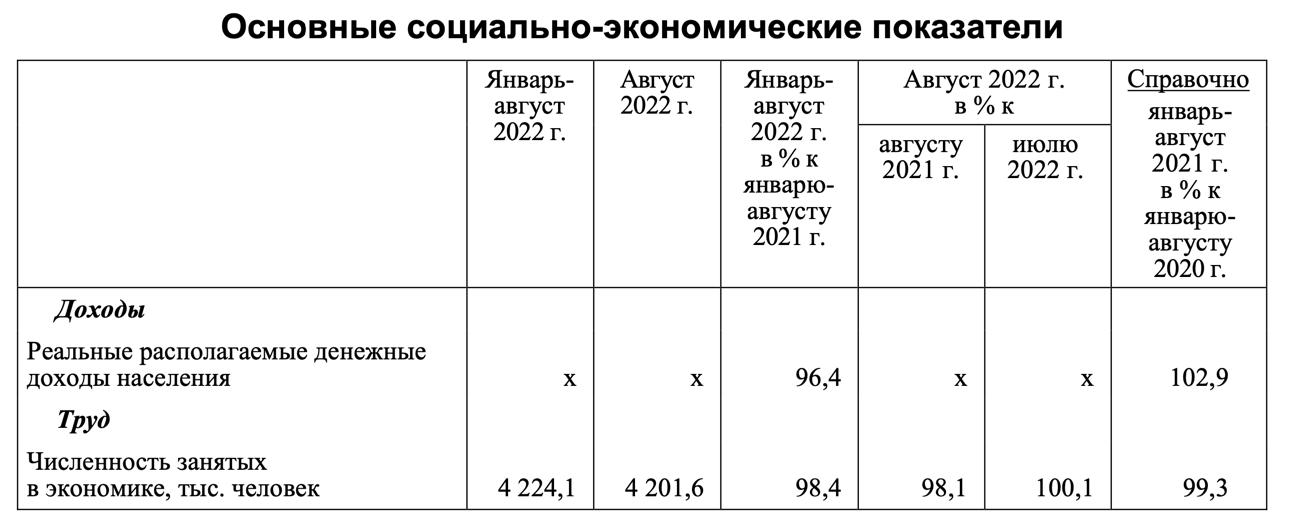
\includegraphics[scale=0.55]{..//images/img}
    }

    \plush{%
        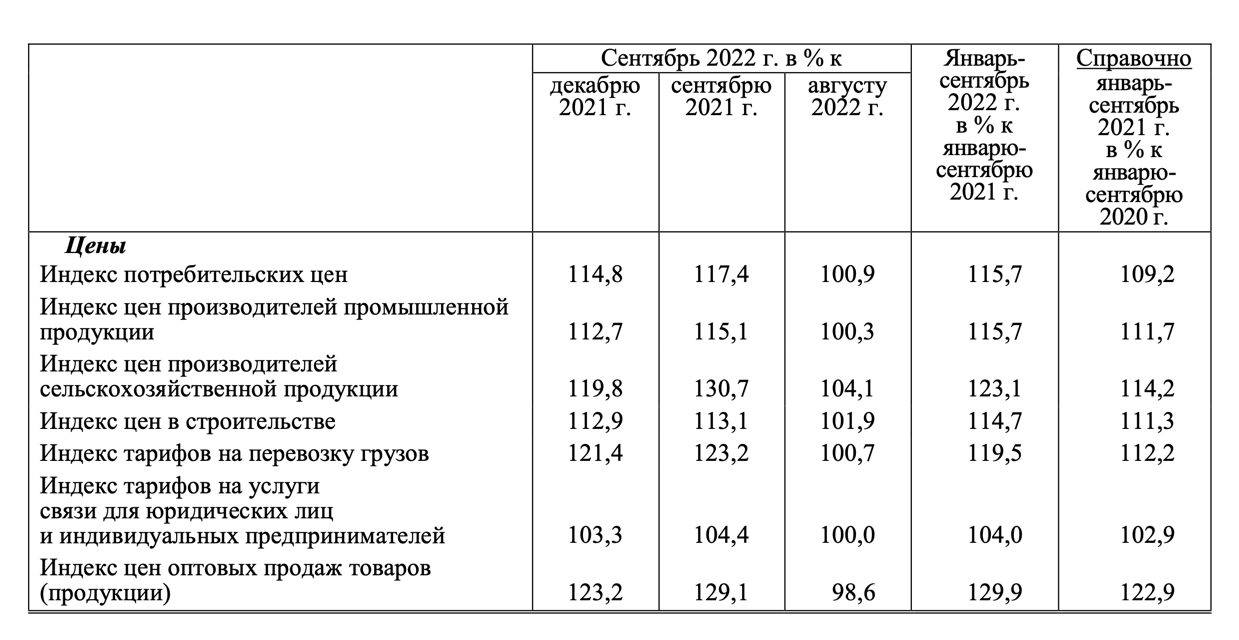
\includegraphics[scale=0.55]{..//images/img_1}
    }

    \plush{%
        \innoSection{Социально-экономическое развитие в РБ}
        \\
        \footnotesize{
            Социально-экономическое развитие – это процесс социально--экономического развития общества.
            Социально-экономическое развитие измеряется такими показателями, как ВВП, ожидаемая продолжительность жизни, грамотность и уровень занятости.
        }
    }

    \plush{%
        \innoSection{2022/2025/2030}
    }

    \plush{%
        \innoSection{Основные проблемы}
    \begin{enumerate}
        \item Высокие цены на сырье и материалы;
        \item санкции;
        \item низкая платежеспособность.
    \end{enumerate}
    }

    \plush[4]{%
        \begin{center}
        {\fontsize{90}{80}\selectfont @h1alexbel}
        \end{center}
    }

    \plush{%
        \innoQR[3in]{https://h1alexbel.github.io/cw-macroeconomics22/}\par
    }

    \plush[4]{%
        \begin{center}
        {\fontsize{90}{80}\selectfont Q\&A}
        \end{center}
    }

\end{document}